%%%%%%%%%%%%%%%%%%%%%%%%%%%%%%%%%%%%%%%%%
% Beamer Presentation
% LaTeX Template
% Version 1.0 (10/11/12)
%
% This template has been downloaded from:
% http://www.LaTeXTemplates.com
%
% License:
% CC BY-NC-SA 3.0 (http://creativecommons.org/licenses/by-nc-sa/3.0/)
%
%%%%%%%%%%%%%%%%%%%%%%%%%%%%%%%%%%%%%%%%%

%----------------------------------------------------------------------------------------
%	PACKAGES AND THEMES
%----------------------------------------------------------------------------------------

\documentclass[UTF8,aspectratio=169,12pt]{ctexbeamer}

\usepackage{hyperref}
\hypersetup{
	colorlinks=true,
	linkcolor=red,
	anchorcolor=blue,
	citecolor=green
}

\mode<presentation> {
	
	% The Beamer class comes with a number of default slide themes
	% which change the colors and layouts of slides. Below this is a list
	% of all the themes, uncomment each in turn to see what they look like.
	
	%\usetheme{default}
	%\usetheme{AnnArbor}
	%\usetheme{Antibes}
	%\usetheme{Bergen}
	%\usetheme{Berkeley}
	%\usetheme{Berlin}
	%\usetheme{Boadilla}
	%\usetheme{CambridgeUS}
	%\usetheme{Copenhagen}
	%\usetheme{Darmstadt}
	%\usetheme{Dresden}
	%\usetheme{Frankfurt}
	%\usetheme{Goettingen}
	%\usetheme{Hannover}
	%\usetheme{Ilmenau}
	%\usetheme{JuanLesPins}
	%\usetheme{Luebeck}
	\usetheme{Madrid}
	%\usetheme{Malmoe}
	%\usetheme{Marburg}
	%\usetheme{Montpellier}
	%\usetheme{PaloAlto}
	%\usetheme{Pittsburgh}
	%\usetheme{Rochester}
	%\usetheme{Singapore}
	%\usetheme{Szeged}
	%\usetheme{Warsaw}
	
	% As well as themes, the Beamer class has a number of color themes
	% for any slide theme. Uncomment each of these in turn to see how it
	% changes the colors of your current slide theme.
	
	%\usecolortheme{albatross}
	%\usecolortheme{beaver}
	%\usecolortheme{beetle}
	%\usecolortheme{crane}
	%\usecolortheme{dolphin}
	%\usecolortheme{dove}
	%\usecolortheme{fly}
	%\usecolortheme{lily}
	%\usecolortheme{orchid}
	%\usecolortheme{rose}
	%\usecolortheme{seagull}
	%\usecolortheme{seahorse}
	%\usecolortheme{whale}
	%\usecolortheme{wolverine}
	
	%\setbeamertemplate{footline} % To remove the footer line in all slides uncomment this line
	%\setbeamertemplate{footline}[page number] % To replace the footer line in all slides with a simple slide count uncomment this line
	
	%\setbeamertemplate{navigation symbols}{} % To remove the navigation symbols from the bottom of all slides uncomment this line
}

\usepackage{graphicx} % Allows including images
\graphicspath{{./figs/}}
\usepackage{booktabs} % Allows the use of \toprule, \midrule and \bottomrule in tables
\usepackage{longtable}
\usepackage{xcolor}
\usepackage{minted}
\usepackage{listings}
\lstset{numbers=left, %设置行号位置
	numberstyle=\tiny, %设置行号大小
	keywordstyle=\color{blue}, %设置关键字颜色
	commentstyle=\color[cmyk]{1,0,1,0}, %设置注释颜色
	frame=single, %设置边框格式
	escapeinside=``, %逃逸字符(1左面的键),用于显示中文
	%breaklines, %自动折行
	extendedchars=false, %解决代码跨页时,章节标题,页眉等汉字不显示的问题
	xleftmargin=2em,xrightmargin=2em, aboveskip=1em, %设置边距
	tabsize=4, %设置tab空格数
	showspaces=false %不显示空格
}
% Fonts
% \usepackage{libertine}
% \setmonofont{Courier}
%\setCJKsansfont[ItalicFont=Noto Serif CJK SC Black, BoldFont=Noto Sans CJK SC Black]{Noto Sans CJK SC}


%----------------------------------------------------------------------------------------
% TITLE PAGE
%----------------------------------------------------------------------------------------

\title[第18讲]{第十八讲 :文件系统实例} % The short title appears at thse bottom of every slide, the full title is only on the title page
\subtitle{第1节:系统可靠性概述}
\author{向勇、陈渝、李国良} % Your name
\institute[清华大学] % Your institution as it will appear on the bottom of every slide, may be shorthand to save space
{
  清华大学计算机系 \\ % Your institution for the title page
  \medskip
  \textit{xyong,yuchen,liguoliang@tsinghua.edu.cn} % Your email address
}
\date{\today} % Date, can be changed to a custom date

\begin{document}

\begin{frame}
\titlepage % Print the title page as the first slide
\end{frame}

%----------------------------------------------
\begin{frame}
\frametitle{提纲} % Table of contents slide, comment this block out to remove it
\tableofcontents % Throughout your presentation, if you choose to use \section{} and \subsection{} commands, these will automatically be printed on this slide as an overview of your presentation

\begin{figure}
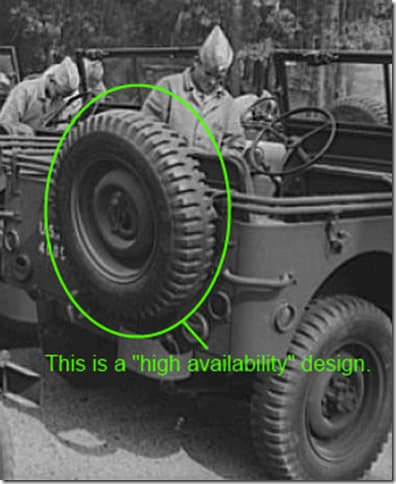
\includegraphics[width=0.2\linewidth]{figs/ha.jpg}
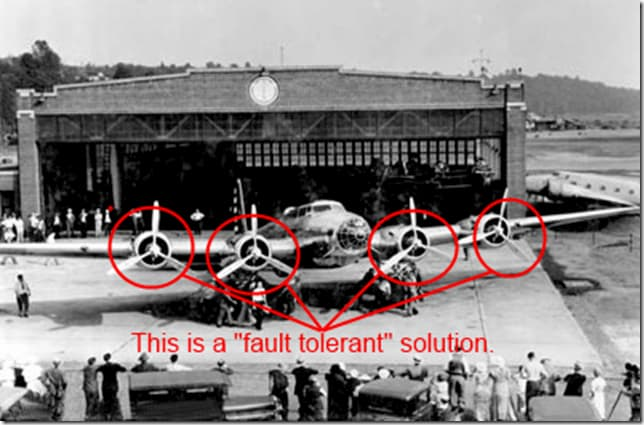
\includegraphics[width=0.37\linewidth]{figs/ft.jpg}
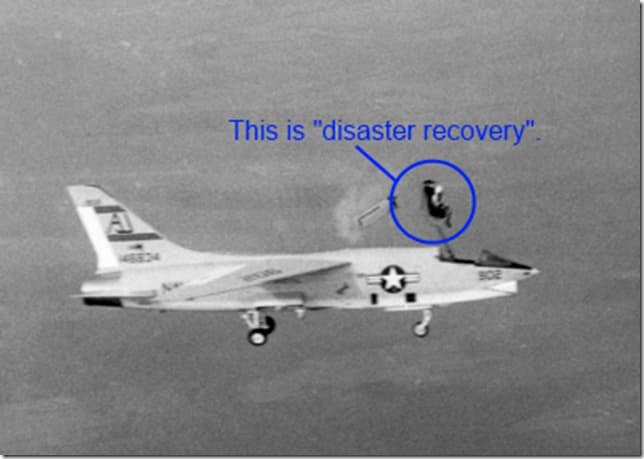
\includegraphics[width=0.34\linewidth]{figs/dr.jpg}
\end{figure}
\end{frame}
%----------------------------------------------
%%  PRESENTATION SLIDES
%----------------------------------------------
\section{第1节:系统可靠性概述} % Sections can be created in order to organize your presentation into discrete blocks, all sections and subsections are automatically printed in the table of contents as an overview of the talk
%----------------------------------------------
\subsection{高可用(High Availability,HA)} % A subsection can be created just before a set of slides with a common theme to further break down your presentation into chunks
%----------------------------------------------
\begin{frame}[fragile]
    \frametitle{高可用(High Availability,HA)}
%    \framesubtitle{xxxx}
%% itemize
\begin{itemize}
    \item 高可用目的:当系统发生故障时,实现快速恢复 \pause
    \item 高可用指标
\begin{itemize}
    \item 4个9: 99.99\%时间可服务,即不可服务时间365*24*60*0.01\%=52.56分钟
    \item 5个9: 99.999\%时间可服务,即不可服务时间365*24*60*0.001\%=5.256分钟
    \item 6个9: 99.9999\%时间可服务,不可服务时间365*24*60*0.0001\%=0.5256分钟
\end{itemize} \pause
    \item 高可用实现手段: 
 \begin{itemize}
    \item 硬件冗余:多台机器备份、故障自检测;纠错码
    \item 软件冗余:多套软件备份:主备,两地三中心,跨城市多活
    \item 自监控、自诊断技术
    \item 恢复设计方案
\end{itemize} 
\end{itemize}
\end{frame}


\begin{frame}[fragile]
    \frametitle{可用性 Availability  vs 可靠性 Reliability}
%    \framesubtitle{xxxx}
%% itemize
\begin{itemize}
    \item 可靠性:在规格允许条件下,系统执行能力。例如网络故障,系统不出现故障。
   \begin{itemize}
    \item 可靠性是指系统可以无故障地持续运行,是一个持续的状态
    \item 如果一个系统从来不崩溃,但是每年要停机两星期,那么它是高度可靠的,但是可用性只有96\%。
   \end{itemize}
   \item 可用性:软件系统在投入使用时,实现其指定系统功能的概率
\begin{itemize}
    \item 在任何给定的时刻都能工作
    \item 如果系统在每小时崩溃1ms,那么它的可用性就超过99.9999\%,但它高度不可靠
\end{itemize}
\end{itemize}
\end{frame}


\begin{frame}[fragile]
    \frametitle{高可靠性指标}
%    \framesubtitle{xxxx}
%% itemize
\begin{itemize}
    \item 平均无故障时间(Mean Time To failures,MTTF) 
\begin{itemize}
    \item 指系统无故障运行的平均时间
    \item 计算方法是:总的正常运行时间/故障次数
    \item 该值越大,表示系统的可靠性越高
\end{itemize} \pause
    \item 平均修复时间(Mean Time To Repair,MTTR) 
 \begin{itemize}
    \item 系统从发生故障到维修结束之间的时间段的平均值
    \item 计算方法是:总的故障时间/故障次数
    \item 该值越小,表示易恢复性越好
\end{itemize}  \pause
 \item 平均失效间隔(Mean Time Between Failure,MTBF) 
 \begin{itemize}
    \item 系统周期性运行至故障至故障处理的全程时间段的平均值
    \item 计算方法是:系统运行至故障处理全程时间/故障次数来表示
    \item 该值越大,可靠性越高,正确工作能力越强
\end{itemize}  
\end{itemize}
\end{frame}





\subsection{容错(Fault Tolerant,FT)} % A subsection can be created just before a set of slides with a common theme to further break down your presentation into chunks
%----------------------------------------------
\begin{frame}[fragile]
    \frametitle{容错(Fault Tolerant,FT)}
%    \framesubtitle{xxxx}
%% itemize
\begin{itemize}
    \item 容错目的:当系统发生故障时,仍可以继续运行,做到零宕机时间。但运行水平可能有所下降(例如只读、最小服务模式) \pause
    \item 容错方法: 
 \begin{itemize}
    \item 故障检测,故障诊断,故障恢复
    \item 冗余设计
    \item 检查点技术checkpoint(从上次检查点恢复)
\end{itemize}  
\end{itemize}
\end{frame}



\subsection{容灾(Disaster Recovery,DR)} % A subsection can be created just before a set of slides with a common theme to further break down your presentation into chunks
%----------------------------------------------
\begin{frame}[fragile]
    \frametitle{容灾(Disaster Recovery,DR)}
%    \framesubtitle{xxxx}
%% itemize
\begin{itemize}
    \item 容灾目的:当系统发生重大灾难时,按照恢复计划挽救数据、恢复业务,力争业务不被中断 \pause
    \item 容灾指标: 
 \begin{itemize}
    \item RPO(Recovery Point Objective):恢复数据的时间点和最新数据的时间点之间的差值;RPO=0意味数据无丢失
    \item RTO (Recovery Time Objective):从服务停止到服务恢复所需时间;RTO=0意味无宕机时间
    \item 完美系统希望RPO=0,RTO=0
\end{itemize}  \pause
   \item 容灾方法:
 \begin{itemize}
    \item 备份恢复:定期备份数据,根据数据恢复
    \item 冗余设计:多副本,全球多副本
\end{itemize} 
\end{itemize}
\end{frame}


\subsection{高可靠系统设计思路} % A subsection can be created just before a set of slides with a common theme to further break down your presentation into chunks
%----------------------------------------------
\begin{frame}[fragile]
    \frametitle{高可靠系统设计思路}
\begin{itemize}
    \item 冗余设计(软件、硬件、带宽冗余)
    \item 快速恢复设计(无状态设计)
    \item 容错、灾备
    \item 隔离(进程、状态、租户)
    \item 过载保护(限流、熔断、有损服务)
    \item 错误重试策略,避免流量风暴
    \item 去关键路径、去中心化、避免单点故障
    \item 负载均衡(load balance)
    \item 看门狗设计
    \item 安全编码
\end{itemize} 
\end{frame}



\end{document}




















\iffalse
%----------------------------------------------
% ###   18.1  File Allocation Table (FAT)
% 
% #### FAT Volume
% 
% ##### File Allocation Table (FAT)
% 
% %% itemize
%     \begin{itemize}
%         \item xx
%     \end{itemize}
% - A simple file system originally **designed for small disks and simple folder structures**. 
% - The FAT file system is named for its method of organization, the **file allocation table**, which resides at the beginning of the volume.
% - To protect the volume, two copies of the table are kept, in case one becomes damaged.
% - **The file allocation tables and the root folder must be stored in a fixed location** so that the files needed to start the system can be correctly located.
% 
%----------------------------------------------
\begin{frame}[fragile]
    \frametitle{Structure of a FAT Volume}
%    \framesubtitle{xxxx}
    %% figure
        \begin{figure}
        \includegraphics[width=1.0\linewidth]{figs/FAT-volume.png}
    %   \caption{xxxx}
        \end{figure}
        %% itemize
    \begin{itemize}
        \item Boot sector \pause
        \item FAT1
        \item FAT2
        \item Root directory \pause
        \item Other directories and all files
    \end{itemize}
\end{frame}
%----------------------------------------------
% ##### Structure of a FAT Volume
% 
% %% itemize
%     \begin{itemize}
%         \item xx
%     \end{itemize}
% - Boot sector
% - FAT1
% - FAT2
% - Root directory
% - Other directories and all files
% 
% %% figure
%   \begin{figure}
%   \includegraphics[width=0.8\linewidth]{test}
%   \caption{xxxx}
%   \end{figure}
% ![FAT-volume](figs/FAT-volume.png)
% 
%----------------------------------------------
\begin{frame}[fragile]
    \frametitle{Differences Between FAT Systems}
%    \framesubtitle{xxxx}
%% figure
    \begin{figure}
  \includegraphics[width=0.95\linewidth]{figs/FAT-version.png}
% \caption{xxxx}
  \end{figure} \pause

%% itemize
    \begin{itemize}
        \item FAT32 is a derivative of the File Allocation Table (FAT) file system that supports drives with over 2GB of storage.
        \item FAT32 drives can contain more than 65,526 clusters and results in more efficient space allocation on the FAT32 drive.
    \end{itemize}
\end{frame}
%----------------------------------------------
% ##### Differences Between FAT Systems
% 
% %% figure
%   \begin{figure}
%   \includegraphics[width=0.8\linewidth]{test}
%   \caption{xxxx}
%   \end{figure}
% ![FAT-version](figs/FAT-version.png)
% 
% %% itemize
%     \begin{itemize}
%         \item xx
%     \end{itemize}
% - FAT32 is a derivative of the File Allocation Table (FAT) file system that supports drives with over 2GB of storage.
% - FAT32 drives can contain more than 65,526 clusters and results in more efficient space allocation on the FAT32 drive.
% 
%----------------------------------------------
\subsection{File Allocation System} % A subsection can be created just before a set of slides with a common theme to further break down your presentation into chunks
%----------------------------------------------
\begin{frame}[fragile]
    \frametitle{Example of File Allocation Table}
%    \framesubtitle{xxxx}
%% figure
    \begin{figure}
  \includegraphics[width=0.9\linewidth]{figs/FAT-example.png}
% \caption{xxxx}
  \end{figure}
\end{frame}
%----------------------------------------------
% ##### Example of File Allocation Table
% 
% %% figure
%   \begin{figure}
%   \includegraphics[width=0.8\linewidth]{test}
%   \caption{xxxx}
%   \end{figure}
% ![FAT-example](figs/FAT-example.png)
% 
%----------------------------------------------
\begin{frame}[fragile]
    \frametitle{File Allocation System}
%    \framesubtitle{xxxx}
    The file allocation table contains the following {\color{red}types} of information about each cluster on the volume (see example below for FAT16):

%% itemize
    \begin{itemize}
        \item Unused (0x0000)
        \item Cluster in use by a file \pause
        \item Bad cluster (0xFFF7)
        \item Last cluster in a file (0xFFF8-0xFFFF)
    \end{itemize}
\end{frame}
%----------------------------------------------
% #### File Allocation System
% 
% ##### File Allocation System
% 
% The file allocation table contains the following **types** of information about each cluster on the volume (see example below for FAT16):
% %% itemize
%     \begin{itemize}
%         \item xx
%     \end{itemize}
%  * Unused (0x0000)
%  * Cluster in use by a file
%  * Bad cluster (0xFFF7)
%  * Last cluster in a file (0xFFF8-0xFFFF)
% 
%----------------------------------------------
\begin{frame}[fragile]
    \frametitle{FAT Root Folder}
%    \framesubtitle{xxxx}
    The root folder contains an entry for each file and folder on the root. The only difference between the root folder and other folders is that {\color{red}the root folder is on a specified location} on the disk and {\color{red}has a fixed size} (512 entries for a hard disk, number of entries on a floppy disk depends on the size of the disk).

\end{frame}
%----------------------------------------------
% ##### FAT Root Folder
% 
% The root folder contains an entry for each file and folder on the root. The only difference between the root folder and other folders is that **the root folder is on a specified location on the disk and has a fixed size** (512 entries for a hard disk, number of entries on a floppy disk depends on the size of the disk).
% 
%----------------------------------------------
\begin{frame}[fragile]
    \frametitle{Folder Entry}
%    \framesubtitle{xxxx}
    The Folder Entry includes the following information:

%% itemize
    \begin{itemize}
        \item Name (eight-plus-three characters)
        \item Starting cluster number in the file allocation table (16 bits)
        \item File size (32 bits) \pause
        \item Attribute byte (8 bits worth of information) \pause
        \item Create time (24 bits)
        \item Create date (16 bits)
        \item Last access date (16 bits)
        \item Last modified time (16 bits)
        \item Last modified date (16 bits)
    \end{itemize}
\end{frame}
%----------------------------------------------
% ##### Folder Entry
% 
% The Folder Entry includes the following information:
% %% itemize
%     \begin{itemize}
%         \item xx
%     \end{itemize}
%  * Name (eight-plus-three characters)
%  * Attribute byte (8 bits worth of information, described later in this section)
%  * Create time (24 bits)
%  * Create date (16 bits)
%  * Last access date (16 bits)
%  * Last modified time (16 bits)
%  * Last modified date (16 bits.)
%  * Starting cluster number in the file allocation table (16 bits)
%  * File size (32 bits)
% 
%----------------------------------------------
\subsection{Filenames on FAT Volumes} % A subsection can be created just before a set of slides with a common theme to further break down your presentation into chunks
%----------------------------------------------
\begin{frame}[fragile]
    \frametitle{Long Filenames on FAT Volumes}
%    \framesubtitle{xxxx}
%% itemize
    \begin{itemize}
        \item FAT creates an {\color{red}eight-plus-three name} for the file. In addition to this conventional entry.  \pause
        \item FAT creates {\color{red}one or more secondary folder entries} for the file, one for each 13 characters in the {\color{red}long filename}. Each of these secondary folder entries stores a corresponding part of the long filename in Unicode. \pause
        \item FAT sets the volume, read-only, system, and hidden {\color{red}file attribute bits} of the secondary folder entry to mark it as part of a long filename. 
    \end{itemize}
\end{frame}
%----------------------------------------------
% #### Filenames on FAT Volumes
% 
% ##### Filenames on FAT Volumes
% 
% %% itemize
%     \begin{itemize}
%         \item xx
%     \end{itemize}
% - FAT creates an **eight-plus-three name** for the file. In addition to this conventional entry. 
% - FAT creates **one or more secondary folder entries** for the file, one for each 13 characters in the **long filename**. Each of these secondary folder entries stores a corresponding part of the long filename in Unicode.
% - FAT sets the volume, read-only, system, and hidden **file attribute bits** of the secondary folder entry to mark it as part of a long filename. 
% 
%----------------------------------------------
\begin{frame}[fragile]
    \frametitle{Folder Entries for the long filename}
%    \framesubtitle{xxxx}
%% figure
\begin{figure}
    \includegraphics[width=0.6\linewidth]{figs/FAT-filename.png}
  % \caption{xxxx}
    \end{figure} \pause

    Figure shows all of the folder entries for the file {\color{red}Thequi~1.fox}, which has a long name of {\color{red}The quick brown.fox}. The long name is in Unicode, so each character in the name uses two bytes in the folder entry. The {\color{red}attribute field} for the long name entries has the value {\color{red}0x0F}. The attribute field for the short name is {\color{red}0x20}.
\end{frame}

\fi
%----------------------------------------------
% ##### Folder Entries for the long filename
% 
% Below shows all of the folder entries for the file **Thequi~1.fox**, which has a long name of **The quick brown.fox**. The long name is in Unicode, so each character in the name uses two bytes in the folder entry. The **attribute field** for the long name entries has the value **0x0F**. The attribute field for the short name is **0x20**
% 
% %% figure
%   \begin{figure}
%   \includegraphics[width=0.8\linewidth]{test}
%   \caption{xxxx}
%   \end{figure}
% ![FAT-filename](figs/FAT-filename.png)
%----------------------------------------------
